\subsubsection{\stid{2.10} PROTEAS-TUNE - Bricks} 

\paragraph{Overview}
We have developed a source-to-source stencil framework (``texttt{Bricks}'')
  to address the growing gap between memory and computational performance 
  on pre-exascale systems.
The approach uses standard \texttt{C++} code to express stencil loops, 
  then transforms the code to use a different memory alignment and ghost
  zone region to optimize memory and communication performance specifically
  for that stencil kernel~\cite{P3HPC_Bricks,zhao2019,zhaoMPI2019}.
This also provides an opportunity to inject architecture-specific code
  transformations, that can take advantage of SIMD/SIMT, threading,
  virtual memory layouts, and the variety of parameters that are needed to 
  tune for optimal performance.
This is a powerful paradigm for having both a correct legal code base 
  using standard tools and, in combination with the autotuning tools previously described,
  the ability to achieve portable performance on many different 
  platforms with minimal, auto-generated code transformations.

\paragraph{Key Challenges}
\texttt{Bricks} require three primary ingredients for performance portability:
\\
(1) \textit{Stencil kernel metadata} - including stencil radius,
  dimensionality, neighbor dependencies, and other memory access patterns.
  For example, for communication the optimal layout depends on the
  extent of stencil corner coupling and symmetry or reuse.
\\
(2) \textit{Transformation profitability model} - based on the architecture
  characteristics and benchmarks, determining what transformations could
  improve overall throughput, not just maximize flops or bytes moved. 
  This can also be explored using roofline models, auto-tuning, 
  communication-avoiding techniques, etc.
\\
(3) \textit{Back-end optimizations and benchmarks} - knowing what 
  architecture-specific transformations achieve the best roofline performance, 
  and how to isolate and compare those with a known benchmark problem. 
For example, if there
  are special OS or hardware capabilities, like vectorized \textit{shuffle}, 
  or memory \textit{mmap} or \textit{prefetch}, that are required to obtain
  peak performance.

\begin{wrapfigure}{r}{0.35\textwidth}
\begin{center}
  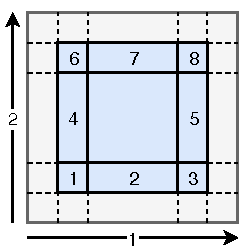
\includegraphics[trim=3mm 5mm 3mm 8mm,width=.33\textwidth]{projects/2.3.2-Tools/2.3.2.10-PROTEAS-YTUNE/Bricks-mpi-parts.pdf}
\end{center}
  \caption{\texttt{Bricks} can be used to map memory onto regions that
  minimize ghost zone packing and MPI message count (2D example).}
\end{wrapfigure}

\paragraph{Solution Strategy}
With \texttt{Bricks}, we have developed a data layout library and code 
  generator for both stencil computations and ghost zone communication.
Recent trends in computer architecture that favor computation over data 
  movement incentivize high-order methods.
Paradoxically, high-order codes can be challenging for compilers/optimization 
  to attain high performance.  
\texttt{Bricks} enable high performance and make fine-grained data reuse and 
  memory access information known at compile time.  
The SIMD code generation achieves performance portability
  for high-order stencils for both CPUs with wide SIMD units (Intel Knights
  Landing and Skylake) and GPUs (NVIDIA Pascal and Volta).  
Integration with autotuning attains performance that is close to Roofline
  performance bound for both manycore CPU and GPU architectures.

\paragraph{Recent Progress}
For optimization of MPI-based communication on exascale proxy systems, 
  we identified several stencil kernels from applications that
  leverage the tuned kernels from previous milestones, and evaluated their
  strong scaling on Theta (Intel KNL) and Summit (NVIDIA V100 GPUs). 
For most stencil codes, strong scaling is
  limited by the communication of ``ghost zone'' values or exchanged between
  processors and nodes, which is required for iterative algorithms or time
  integrators. 
Because each MPI rank has one or more subdomains with different layouts 
  in memory, this involves ``packing'' before sending – copying a subset of
  local arrays into an MPI message buffer – and then ``unpacking'' 
  (copying buffers to array subset) after receiving data. 
This involves both strided memory access
  and accessing the same array as different messages are sent or received. 
These operations on the ghost zone ``skin'' can introduce significant latency 
  and is a blocking operation that, in the limit of strong scaling, 
  can’t be hidden by overlapping communication and computation. 
We have used our \texttt{Bricks} source-to-source transformation technique to 
  eliminate the cost of MPI packing/unpacking on CPUs and GPUs, which 
  improves strong scaling for block semi-structured applications, is 
  performance-portable, and is directly relevant to applications with many 
  DoF’s per grid point (such as in combustion and multi-physics codes). 
We have also introduced a novel technique on CPU to
  significantly reduce the number of messages, using an indirect mapping 
  of memory to MPI buffers. 


\paragraph{Next Steps}
For FY20, we are extending \texttt{Bricks} to other
  application patterns, including block-structured AMR, chemistry kernels,
  and systems of (non-)linear solvers.
For these, the primary focus will be on investigating the profitability
  models, code transformations, and auto-tuning the kernels.
As more diverse architectures and benchmarks become available within 
  the ECP program (AMD GPU, Intel GPU, NVIDIA Turing), we will develop 
  transformations that provide better porformance portability.
We will be building up to portable \textit{application} performance 
  and load balancing; this is a complex trade-off between all kernels in
  a given code, and will be very application- and architecture-dependent.

  

%\end{document}
